\documentclass[11pt]{article}
\usepackage[utf8]{inputenc}
\usepackage[T1]{fontenc}
\usepackage[margin=1in]{geometry}
\usepackage{amsmath}
\usepackage{tikz}
\usetikzlibrary{arrows.meta}
\usepackage[authoryear,round]{natbib}
\usepackage{indentfirst}
\usepackage{graphicx}
\usepackage{booktabs}
\graphicspath{{../output/}}
\begin{document}

%==============================================
\title{Concentration Effect in Youth Crime}
\author{}
\date{\today}
\maketitle
%==============================================

Note: This is not written in a "paper tone", but more as a report to registry the reasoning and the data
\section{Research question}

\noindent Does the concentration of students leaving school at the same time
affect crime in the short run?

\paragraph{Reduced form.} Did the 2014 change in the schedule of 1st-year EM
classes, which stopped them from leaving school at the same time as the 2nd
and 3rd years, change crime by or against 2nd- and 3rd-year students after
release, in schools that used to release all EM years together?

 \section{Motivation}

School reduces youth crime in two ways: it raises human capital in the long
run \citep{lochner2004}, and it keeps students in a supervised environment, where they can not commit crime 
(incapacitation). But school also brings young people
together, generating networks. \citet{billings2019} studes the effect of school in formation of network using the redrawing of
school boundaries in Charlotte-Mecklenburg in 2002. They find that one standard
deviation more same-school, same-grade, same-race and same-gender peers living
within 1 km raises the probability of arrest at ages 16--21 by 3.9 percentage
points (23\%). Two students who live within 1 km of each other are 
more likely to be arrested together (in the long-run) if they are assigned to the
same school.

Concentration can also raise crime in the short run, while students are
together. The literature shows evidence of the concentration effects through variation in session-days and the
type of crime. \citet{jacob2003} show that propery crime falls by 14\% on school days, but juvenile
violent crime rises by 28\%, and the violent crime peaks at about 3 p.m.,
when school lets out. The authors arugue that the fall in property crime is an evidence of incapacitation effects,
 and the rise of violent crime is an effect of concentration.  \citet{luallen2006} follows the same line and shows that the
property crime increases
 and violent crime decreases on strike days. 


I believe this is weak evidence of a concentration effect for some reasons.
First, they identify only the net effect of incapacitation and concentration.
The effect of school on violent crime is the sum of incapacitation ($-$) and
concentration ($+$). Since the net effect is positive, concentration
outweighs incapacitation for violent crime. The effect on property crime is the
sum of incapacitation ($-$) and concentration, whose sign is unknown. If we
assume it is non-negative, the negative net effect  means that
incapacitation outweighs concentration for property crime. Under these sign
assumptions, they identify only the lower bound of the concentration effect. 


Second, the source of variation is a whole day without school, which changes
substantially what students do during the day, not only how many other students
they meet. The changes in property and violent crime can therefore reflect the
different opportunities students face on an ``atypical'' day: the same student
can change which crime they commit. For example, a student who would have
fought at school (violent crime) may instead shoplift at a mall (property
crime), because a free day leaves time to comute to the mall that is far away.
 If students substitute across crimes in this way, the type of
crime does not  identify whether incapacitation or concentration is at work. 

Third (and less severe), although \citet{jacob2003} argue that the bias of school-reporting by 
estimating the effect of non school hours crimes or crimes that occured out of schools, their effect decrease with their significance. 

Separating concentration from incapacitation is hard. Any policy that changes
when students leave school usually also changes how long they stay there, and
so how much time they spend supervised. This paper uses a source of variation
that changes concentration while keeping school and supervision fixed. 
Two advantages of this paper: incapacitation is held fixed, concentration is measured, not inferred. 
We could have a dose-response of the concetration of the youth (\textcolor{red}{check that, the first spec would be binary})


Understanding the contemporaneous effect of concentration matters for two reasons:
\begin{enumerate}
  \item It is cheap to prevent. If shared release raises crime, staggering bell
        times is a low-cost policy, unlike lengthening the school day or
        reassigning students across schools.
  \item It may feed the long-run effect. If crimes committed together after
        school are where partnerships start, the short-run concentration effect
        is one channel behind the networks documented by \citet{billings2019}. \citet{luallen2006} finds that juveniles who become repeat
        offenders are more likely to commit their first crime on a strike day.
\end{enumerate}


 \section{Mechanisms}

I can think of three mechanisms on which conecetration of youth can increase crime. First, is the numeric concentration of people, second the peer effect and 
third the report. Each of these mechanisms operate in the different manner. 
\begin{enumerate}
      \item[A.] First, the number of people: how many young people are around.
            A concentration of people can increase crime because:
      \begin{enumerate}
            \item there are more interactions, which can help youths
                  coordinate crimes. \citet{jacob2003} find no evidence that
                  school increases the coordination of crime: crimes with
                  several offenders do not respond more to school days. We can
                  test whether the number of crimes committed by more than one
                  student increases.
            \item there are more people who can fight each other. We can test
                  this, but we cannot separate it from old rivalries (the peer
                  effect below).
            \item there is less adult supervision per youth (police, school
                  staff, security guards on the street), as long as the police
                  do not respond to the crowd.
            \item more students can attract offenders, which increases crime
                  against students. We can check whether the number of student
                  victims increases.
      \end{enumerate}
      \item[B.] Second, the peer effect: .
      \begin{enumerate}
            \item \textbf{Learning.} Students can learn from other students.
                  In our main specification, we are measuring the exposition of older students to
                  younger ones so this channel may be weaker in our case. But we can test (long-shot) if there is an increase in crimes
                   committed jointly with a prior offernder and a first-time offender.  Perhaps we do not have enough variation. 
            \item \textbf{Recruitment.} If a 3rd-year
                  student pulls 1st-year students into a theft, the 3rd-year
                  student's own crime also increases, because they offend
                  together. We can test this with crimes committed by mixed-grade
                  groups.             
            \item \textbf{Status.} Older students may act out/show off to
                  impress younger ones. 
            \item \textbf{Within student rivalries.} Students can fight because of their
                  rivalries, including hazing of 1st-year students by older
                  students. This predicts fights
                 across grades, with older offenders and younger
                  victims. We can test this. 
      \end{enumerate}
            \item[C.] Third, policing and reporting (I am not sure if we treat this as a mechanism or a confounder... )

            \begin{itemize}
                  \item \textbf{Reporting.} A crowd can change the share of
                        crimes that reach the police, in either direction.
                        It can decrease reporting:                       offenders are harder to identify in a crowd and
                         each witness expects
                        someone else to call
                   Also, fights between students that would otherwise happen away from the school
may happen at the school gate when students are released together. There, the
school is more likely to handle them as a discipline matter, so they are less
likely to be reported to the police.
                         It can increase reporting: there are
                        more witnesses and more phones to film or call.
                  \item \textbf{More police.} When students leave together,
                        the police can respond with more patrols at the school
                        gate. This has two effects: more
                        police can deter crime (a real change in
                        behavior), and more police can detect more, 
            \end{itemize}
            We can test for these channels by checking whether, with shared
            release:
            \begin{enumerate}
                  \item the average time between the crime and the arrival of
                        the police (or the report) changes;
                  \item the share of crimes in which the police are already at
                        the scene, or arrest the offender in the act
                        (\emph{flagrante}), increases;
                  \item the share of incidents started by the police (patrol)
                        rather than by a call from a victim or witness changes;
                  \item serious crimes, which are reported whoever is watching
                       , respond in the same way as
                        minor crimes. If only minor crimes respond, the effect
                        is more likely to come from reporting.
            \end{enumerate}
\end{enumerate}

\section{Further analysis/Heterogenous}
We can also investigate:
\begin{enumerate}
  \item \textbf{Displacement.} Does staggered release reduce crime, or only
        shift it to other times and days? \citet{jacob2003} and \citet{luallen2006} find no temporal displacement of violent crime (leads and lags,
        and weekly and monthly totals). We can run the same tests.
  \item \textbf{Place.} Where does concentration-driven crime happen: at the
        school gate, or along the routes between school and home?
  \item \textbf{Type of crime.} Is the effect driven by fights between students
        (assaults with young victims) or by property crime? Is it larger for
        crimes with several juvenile offenders? \citet{jacob2003} find no
        evidence that school helps juveniles coordinate crimes. \citet{billings2019} find that partnerships are common among older
        youth.
      \item Crime against students
      \item Powered effect of concentration: if have two shifts in the smae school. The program makes students go earlier in the school in the afternoon shift (starts at \_)


\end{enumerate}



\section{Population of Study}

\begin{itemize}
  \item \textbf{Population.} Students in the 2nd and 3rd years of high school
        (EM) in state schools in Minas Gerais that offer all three years of EM.
  \item \textbf{Treatment.} The class is released at the same time as the
        1st-year EM classes of the same school and shift. A continuous version
        is the number of 1st-year students released within $X$ minutes of the
        class.
  \item \textbf{Outcome.} Crime committed by (and against) 2nd- and 3rd-year
        students after release, near the school and in the minutes after the
        bell.
\item Level of analysis: school
\end{itemize}

\paragraph{Sample.} State schools in Minas Gerais with at least one 1st-, 2nd-
or 3rd-year EM class in 2013, excluding the schools of the \emph{Reinventando o
Ensino M\'edio} pilot (2012 and 2013). Table~\ref{tab:escolas_2013} describes
the sample. The analysis uses the 1,325 of these schools that, in 2013, had EM
classes in the morning and none in the afternoon; they may also have night
classes (Table~\ref{tab:turnos}).

\begin{table}[htbp]
\centering
\caption{State schools with high school (EM) in Minas Gerais, 2013.}
\label{tab:escolas_2013}

\begin{tabular}{lrr}
\toprule
State schools with high school, 2013 & N & \%\\
\midrule
1. Schools with 1st, 2nd and 3rd years of HS & 2,174 & 100.0\\
2. Pilot schools & 132 & 6.1\\
3. Schools with afternoon HS classes & 547 & 25.2\\
4. Schools with different release times within grade & 95 & 4.4\\
5. Schools without morning HS classes & 197 & 9.1\\
Sample (1 - 2 - 3 - 4 - 5) & 1,203 & 55.3\\
\bottomrule
\end{tabular}

\par\medskip
\begin{minipage}{0.9\textwidth}
\footnotesize \emph{Notes:} Schools with at least one 1st-, 2nd- or 3rd-year
EM class (regular, integrated or teacher training) in 2013. The sample excludes
the schools of the \emph{Reinventando o Ensino M\'edio} pilot (2012 and 2013).
Percentages are relative to the sample. Duration rows: change in the mean
duration of 1st-year classes from 2013 to 2014 in at least one shift of the
school; unchanged means the same mean duration in every shift with 1st-year
classes in both years. Morning: classes starting before 12:00; afternoon:
classes starting between 12:00 and 14:00. Release times are compared within the
same grade and shift, morning and afternoon only. Average classes per grade:
mean over school $\times$ grade.
\end{minipage}
\end{table}

\begin{table}[htbp]
\centering
\caption{Sample schools by the shift of their EM classes, 2013.}
\label{tab:turnos}

\begin{tabular}{lrrr}
\toprule
Non-pilot schools by EM shift, 2013 & N & \% & Also night EM\\
\midrule
Non-pilot schools & 2,077 & 100.0 & 1,344\\
Only morning & 1,325 & 63.8 & 823\\
Only afternoon & 146 & 7.0 & 66\\
Morning and afternoon & 405 & 19.5 & 254\\
Neither (night only or no time) & 201 & 9.7 & 201\\
\bottomrule
\end{tabular}

\par\medskip
\begin{minipage}{0.9\textwidth}
\footnotesize \emph{Notes:} Sample of Table~\ref{tab:escolas_2013}. Shift of
the 1st-, 2nd- and 3rd-year EM classes: morning, classes starting before
12:00; afternoon, classes starting between 12:00 and 14:00; night, classes
starting after 14:00. Only morning: at least one morning class and no afternoon
class; only afternoon: the reverse. The rows can also have night classes; the
last column counts them. Percentages are relative to the sample.
\end{minipage}
\end{table}

\begin{table}[htbp]
\centering
\caption{Sample schools that release the 1st year together with the 2nd and
3rd years, 2013--2015.}
\label{tab:saida_junto}

\begin{tabular}{lrrr}
\toprule
Year & Comparable schools & Release within 5 min & \%\\
\midrule
2013 & 1,144 & 1,134 & 94.3\\
2014 & 1,169 & 322 & 26.8\\
2015 & 1,180 & 1,077 & 89.5\\
\bottomrule
\end{tabular}

\par\medskip
\begin{minipage}{0.9\textwidth}
\footnotesize \emph{Notes:} Sample of Table~\ref{tab:escolas_2013}. For each
school, year and shift (morning or afternoon), difference between the mean
release time of 1st-year classes and the mean release time of 2nd- and 3rd-year
classes. Release within 5 min: the difference is 5 minutes or less in at least
one shift. Comparable schools: schools with 1st-year and 2nd- or 3rd-year
classes in the same shift in that year. Percentages are relative to the sample.
\end{minipage}
\end{table}

\section{Main Identification Strategy}

\subsection{Motivation for the Identification Strategy}

\paragraph{The naive comparison.} The simplest design compares schools that
release the three EM years together with schools that release each year at a
different time. But release times are not random. There are confounders at school, individual, time of day levels. 

\emph{School level.}Schools with fewer classes can release
        everyone together, so shared release is more common in smaller schools.
        Smaller schools are in less dense areas with less crime. Staggered times often can come from lack of rooms
        or extra shifts, which are also related to school quality.
 Principals may stagger release
        because of fights at the gate, so treatment responds to past
        violence (PARA CLAUDIA: COLOCAR ESTE PARENTESES EM VERMLEHO check if this reverse causality impact the main specification).


\emph{Individual level.}   Families choose schools, so students in
        small schools with shared release differ from students in large
        schools (income, distance from home, prior behavior).
  \ Schools assign students to
        shifts and classes by age, repetition, behavior. If
        some classes are released at different times, the students in them may
        differ in their risk of crime.

\emph{Time of day.} A different release time is a different clock time, with
different parental supervision, daylight, policing and street activity.

\paragraph{A source of variation: the 2014 change in 1st-year schedules.} In
2014, 1st-year EM classes in state schools in Minas Gerais became about
50 minutes longer, for that year only (bacause of
\emph{Reinventando o Ensino M\'edio}). Morning 1st-year classes
moved their release from 11:20--11:30 to about 12:10--12:20.
 In 2015 the 1st year went back to its previous schedule. PARA CLAUDIA: COLOCAR GRAFICO DE LINHA AQUI



For a 2nd- or 3rd-year student in a school that released all EM years
together, this means:
\begin{itemize}
  \item \textbf{Concentration falls in 2014 and returns in 2015.} The 1st-year
        students no longer leave with them in 2014, and leave with them again
        in 2015.
  \item \textbf{Their own schedule is unchanged.} Start time, class duration
        and release time are the same, so incapacitation (hours in school,
        free time) and clock time are held fixed.
  \item \textbf{The change is set by the state, not by the school.} It does not
        respond to violence at a particular school's gate.
\end{itemize}

\paragraph{Design.} Compare 2nd- and 3rd-year students in schools that shared
release with the 1st year before 2014 (treated: sharing stops in 2014 and
returns in 2015) with students in schools that did not share release (control:
no change), in 2012--2016. The reversal in 2015 is a second test: if crime
falls in 2014 because of lower concentration, it should rise again in 2015.

\begin{itemize}
  \item \textbf{Comparison:} treated vs control schools, before, during and
        after 2014.
  \item \textbf{Unit:} 2nd- and 3rd-year class (or school $\times$ shift)
        $\times$ year.
  \item \textbf{Fixed effects:} school $\times$ shift and year.
  \item \textbf{Identifying assumption:} without the 2014 change, crime around
        the release of 2nd- and 3rd-year students would have evolved in
        parallel in treated and control schools; and the 2014 change affected
        these students only through the number of students released with
        them.
\end{itemize}



\paragraph{Treated and control schools.} The sample is the 1,325 schools with
EM classes in the morning and none in the afternoon in 2013
(Table~\ref{tab:turnos}). The criteria use only their morning classes, in
schools with 1st-, 2nd- and 3rd-year morning classes in 2013 and 2014. Start
time, class duration and release time are the means over the morning classes of
each grade in the school.
\begin{itemize}
  \item \textbf{(i) Shared release in 2013:} the 1st year left at most 5 minutes
        before or after the 2nd year and the 3rd year.
  \item \textbf{(ii) The 1st year leaves later in 2014:} the 1st year left 40
        minutes or more after the 2nd and the 3rd years, and its class duration
        rose by 40 minutes or more from 2013 to 2014.
  \item \textbf{(iii) The 2nd and 3rd years do not change:} same start time and
        same class duration in 2013 and 2014, and so the same release time.
  \item \textbf{Treated:} (i), (ii) and (iii).
  \item \textbf{Control:} (i) and (iii), and in 2014 the 1st year still left at
        most 5 minutes before or after the 2nd and the 3rd years.
\end{itemize}
This control differs from the one in the design above (schools that did not
share release): here, control schools shared release in 2013 and kept sharing
it in 2014. The identifying assumption becomes parallel trends between schools
that changed the 1st-year schedule and schools that did not; it fails if the
reason a school did not change also changes its crime trend.
Table~\ref{tab:tratamento} counts the schools that meet each criterion.

\begin{table}[htbp]
\centering
\caption{Treated and control schools: schools with EM in the morning and not in
the afternoon, 2013.}
\label{tab:tratamento}

\begin{tabular}{lrr}
\toprule
Schools & N & \%\\
\midrule
Sample (Table 1) & 1,431 & 100.0\\
1st, 2nd and 3rd years in the morning, 2013 and 2014 & 1,079 & 75.4\\
(i) Shared release in 2013 & 1,069 & 74.7\\
(ii) 1st year leaves 40+ min later in 2014 & 692 & 48.4\\
(iii) 2nd and 3rd years unchanged & 843 & 58.9\\
Treated: (i), (ii) and (iii) & 573 & 40.0\\
Control: (i) and (iii), still shared in 2014 & 221 & 15.4\\
Other: (i) and (iii), neither & 46 & 3.2\\
\bottomrule
\end{tabular}

\par\medskip
\begin{minipage}{0.9\textwidth}
\footnotesize \emph{Notes:} Only morning: sample schools of
Table~\ref{tab:escolas_2013} with 1st-, 2nd- or 3rd-year EM classes starting
before 12:00 and none starting between 12:00 and 14:00 in 2013
(Table~\ref{tab:turnos}); they may have night classes. The criteria use only
morning classes. Percentages are relative to the only-morning sample. Criteria
(i)--(iii), treated and control as defined in the text. Other: schools that
meet (i) and (iii) but neither (ii) nor the control condition (for example, in
2014 the 1st year leaves between 5 and 40 minutes after the 2nd and 3rd years).
\end{minipage}
\end{table}

\paragraph{Threats.}
\begin{itemize}
  \item \textbf{Treated and control schools differ.} Schools that shared
        release are smaller (see above). Fixed effects absorb level
        differences, but not different trends. Check pre-trends in 2010--2013.
  \item \textbf{The 1st-year students also change.} In 2014 they leave later
        and spend more time in school, so their own crime changes. The outcome
        must be crime by (or against) 2nd- and 3rd-year students, not all
        youth crime near the school.
  \item \textbf{Other changes in 2014.} The policy may have come with other
        changes at the school (activities, staff) that affect all students. In
        addition, Belo Horizonte hosted World Cup matches in June--July 2014,
        with changes to the school calendar and heavy policing, and 2014 was an
        election year. Year fixed effects absorb what is common to all
        schools, but not effects that differ between treated and control
        schools.
  \item \textbf{Some 2nd-year classes also change.} The 3rd-year schedule does
        not change in 2014, but a small share of 2nd-year classes also leaves
        later that year (Figures~\ref{fig:em_series_manha}
        and~\ref{fig:em_series_tarde}). For these classes, the students' own
        release time changes too.
  \item \textbf{Compliance.} Not all schools changed the 1st-year schedule in
        2014 (Tables~\ref{tab:escolas_2013} and~\ref{tab:saida_junto}). Use the
        observed change in each school's schedule, not just the year.
\end{itemize}

\paragraph{Descriptive evidence on the 2014 change.} Table~\ref{tab:escolas_2013}
counts the sample schools whose mean 1st-year class duration rose 50 minutes or
more from 2013 to 2014: 1,135 of 2,076 schools (54.7\%). The sample excludes
the schools of the \emph{Reinventando o Ensino M\'edio} pilot (2012 and 2013),
which may have adopted the change before the rest of the network.

Figure~\ref{fig:em_series_manha} shows that, in the morning, 1st-year classes
moved from 11:20--11:30 to 12:15--12:20 in 2014 only, while 2nd- and 3rd-year
classes kept leaving at 11:20--11:30. Figure~\ref{fig:em_series_tarde} shows the
same in the afternoon: 1st-year classes moved from 17:00--17:30 to
17:50--18:20, while 2nd- and 3rd-year classes kept their release time. In the
earlier sample of the Belo Horizonte metropolitan region, some schools also
moved the afternoon start time earlier in 2014 (from 13:00 to 12:30), for the
2nd year as well as the 1st; this still has to be checked in the current
sample.

Figure~\ref{fig:hist_diff} compares, within each school, the release time of
the 1st year with that of the 2nd and 3rd years in the morning shift. In 2013
and 2015 almost every school releases all EM years at the same time (difference
of zero). In 2014 most schools release the 1st year about 50 minutes after the
2nd and 3rd years: the median difference is 50 minutes, and 1,067 of 1,654
schools have a difference of 40 minutes or more. 450 schools keep releasing all
years together in 2014.

\begin{figure}[ht]
\centering
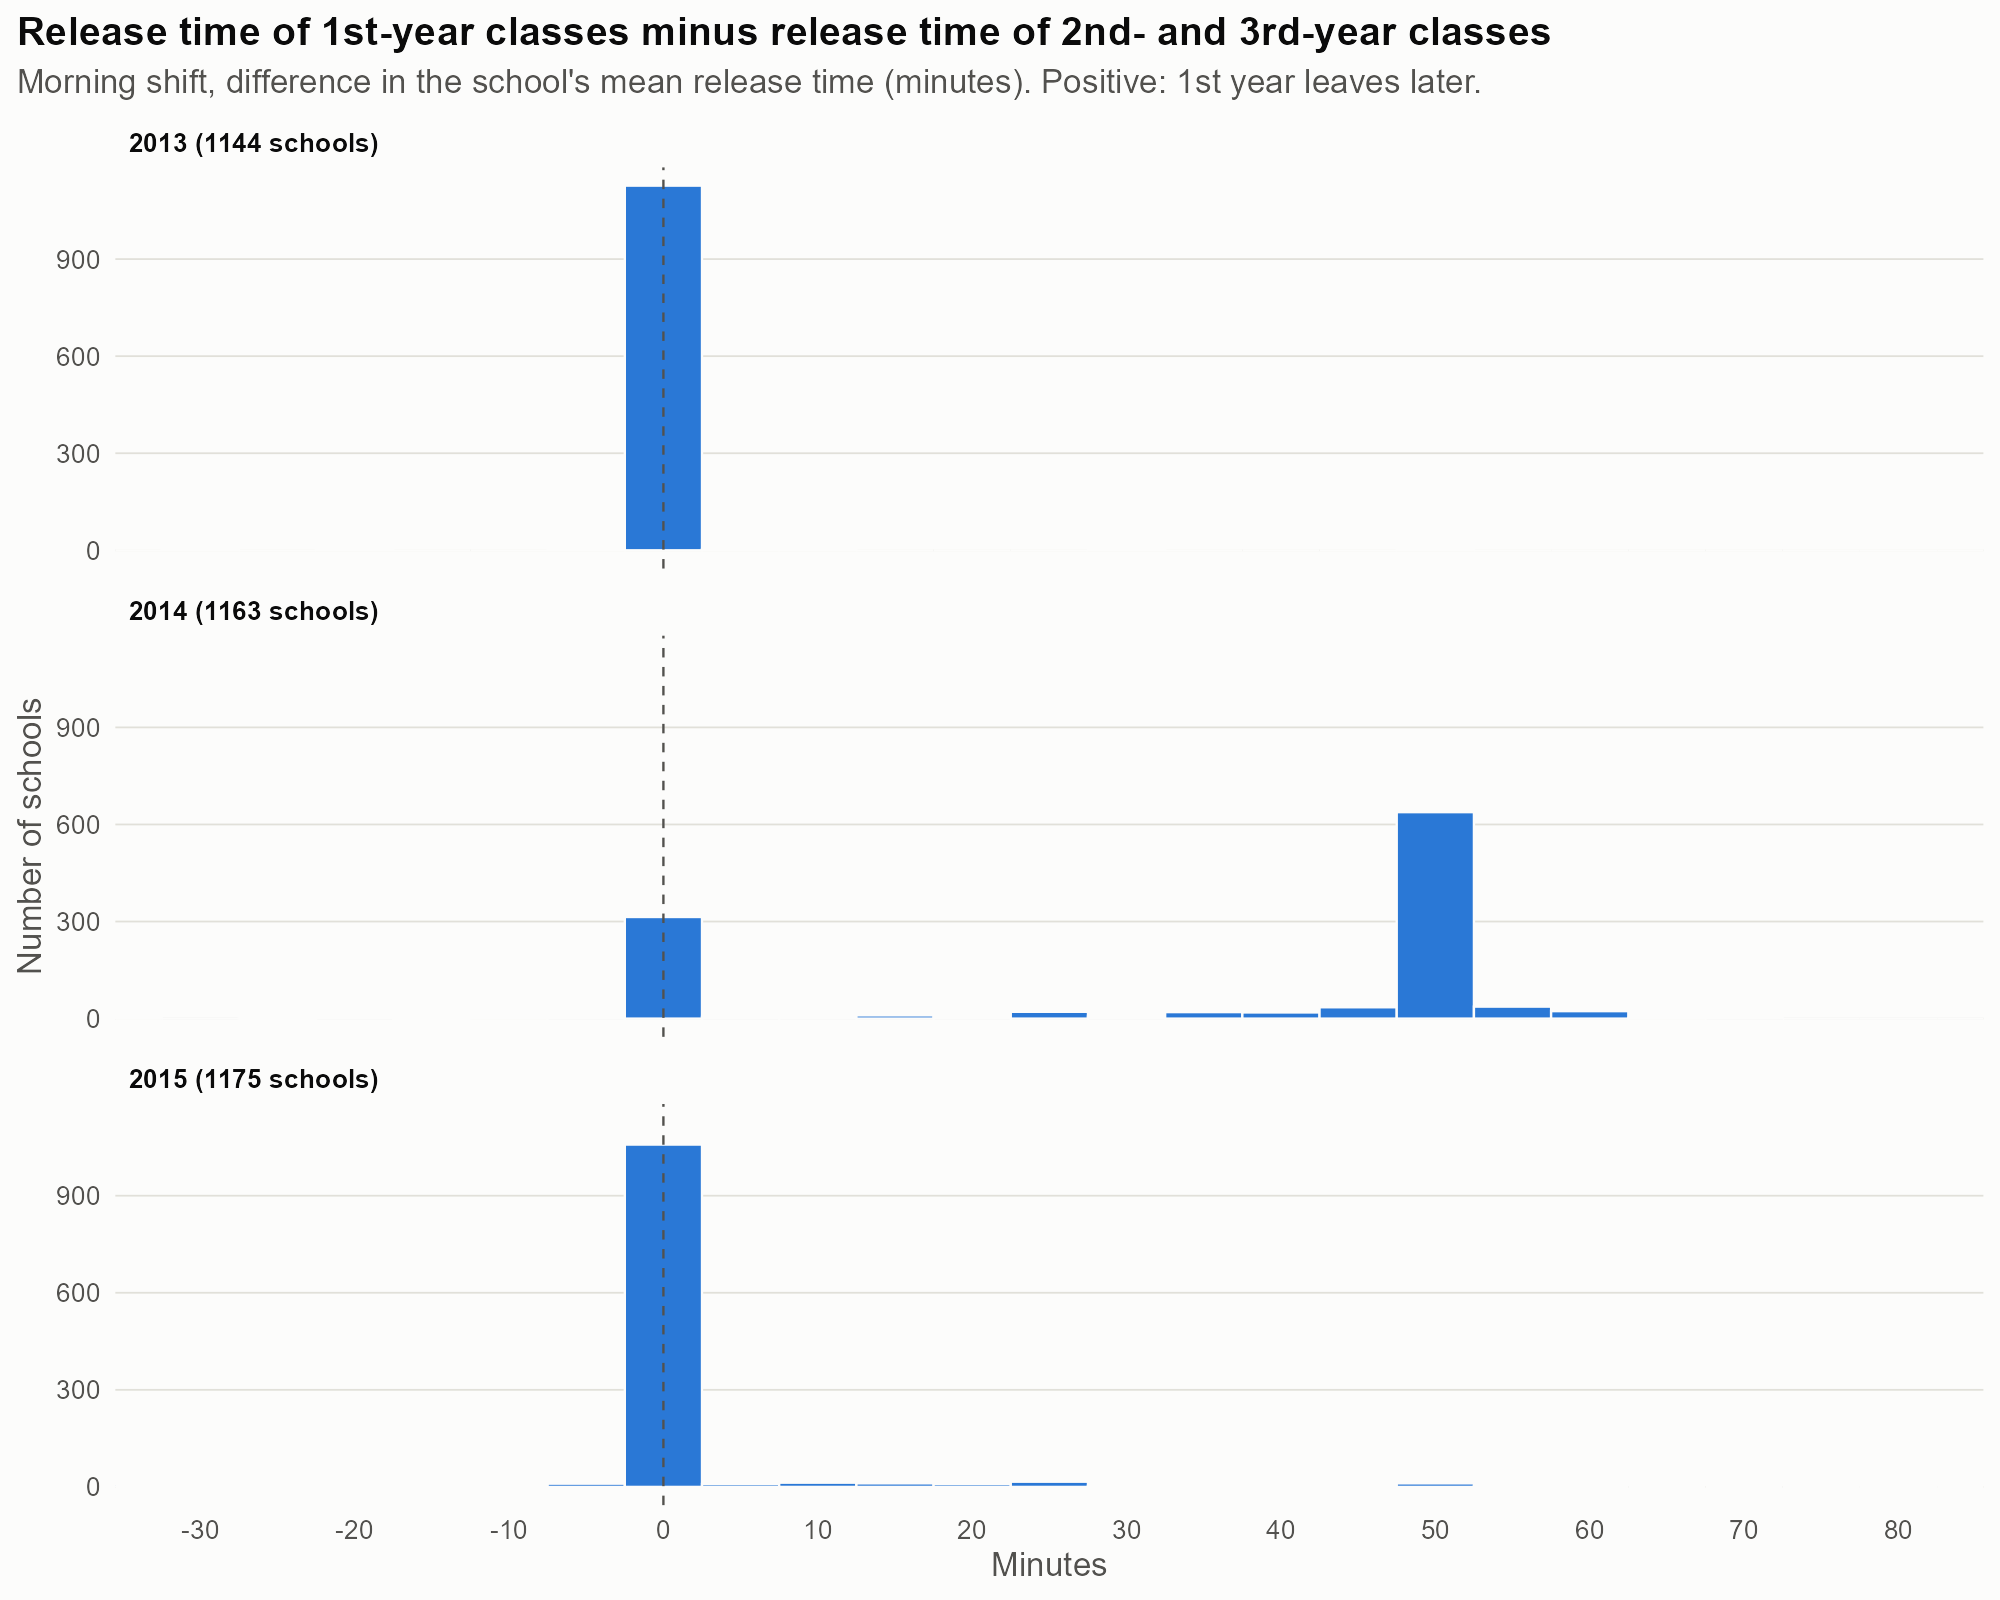
\includegraphics[width=0.9\textwidth]{hist_diff_saida_1em_manha.png}
\caption{Difference, in each school, between the mean release time of 1st-year
EM classes and the mean release time of 2nd- and 3rd-year EM classes, morning
shift (classes starting before 12:00), in 2013, 2014 and 2015. Positive values:
the 1st year leaves later. Sample schools (Table~\ref{tab:escolas_2013}) with
both 1st-year and 2nd- or 3rd-year morning classes in the year. The horizontal
axis is cut at $-30$ and $80$ minutes, which leaves out 15 schools in 2013, 8 in
2014 and 13 in 2015.}
\label{fig:hist_diff}
\end{figure}




\section{Release times by EM grade}

\begin{figure}[htbp]
\centering
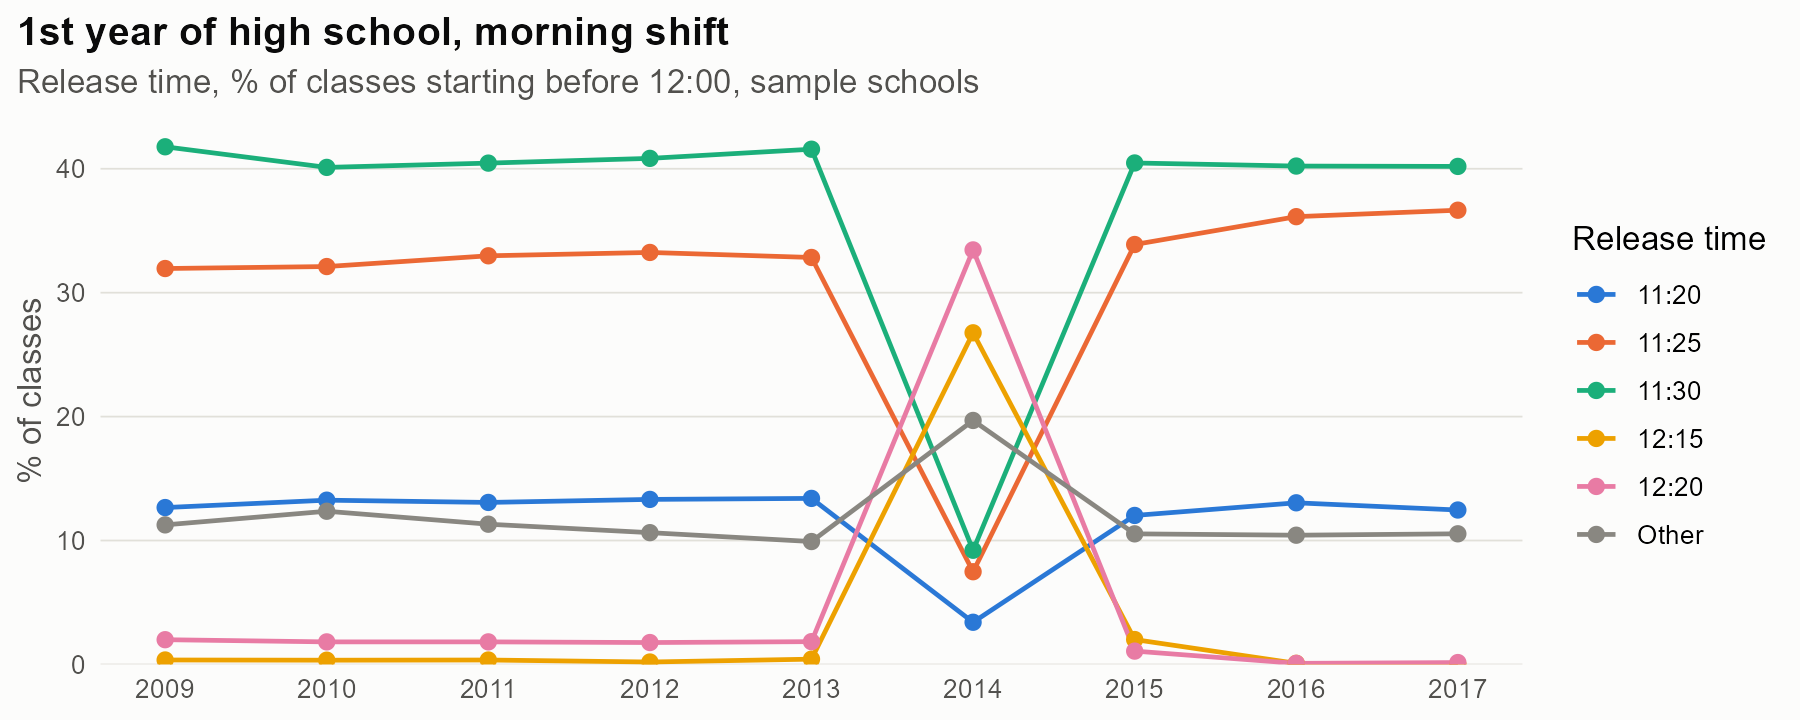
\includegraphics[width=0.85\textwidth]{horarios_em_series_manha_1ano.png}\\[1ex]
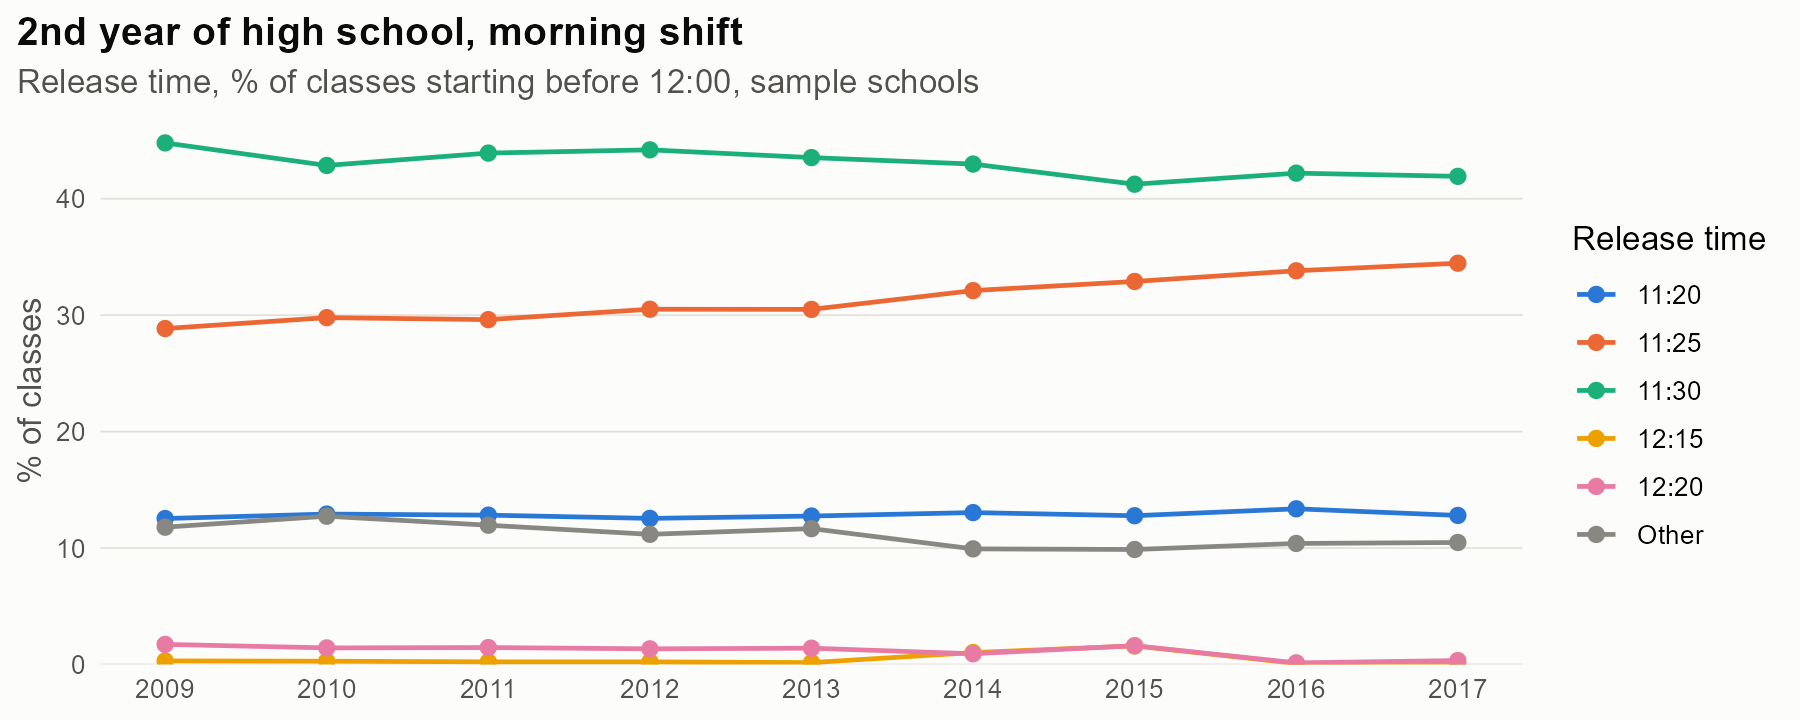
\includegraphics[width=0.85\textwidth]{horarios_em_series_manha_2ano.png}\\[1ex]
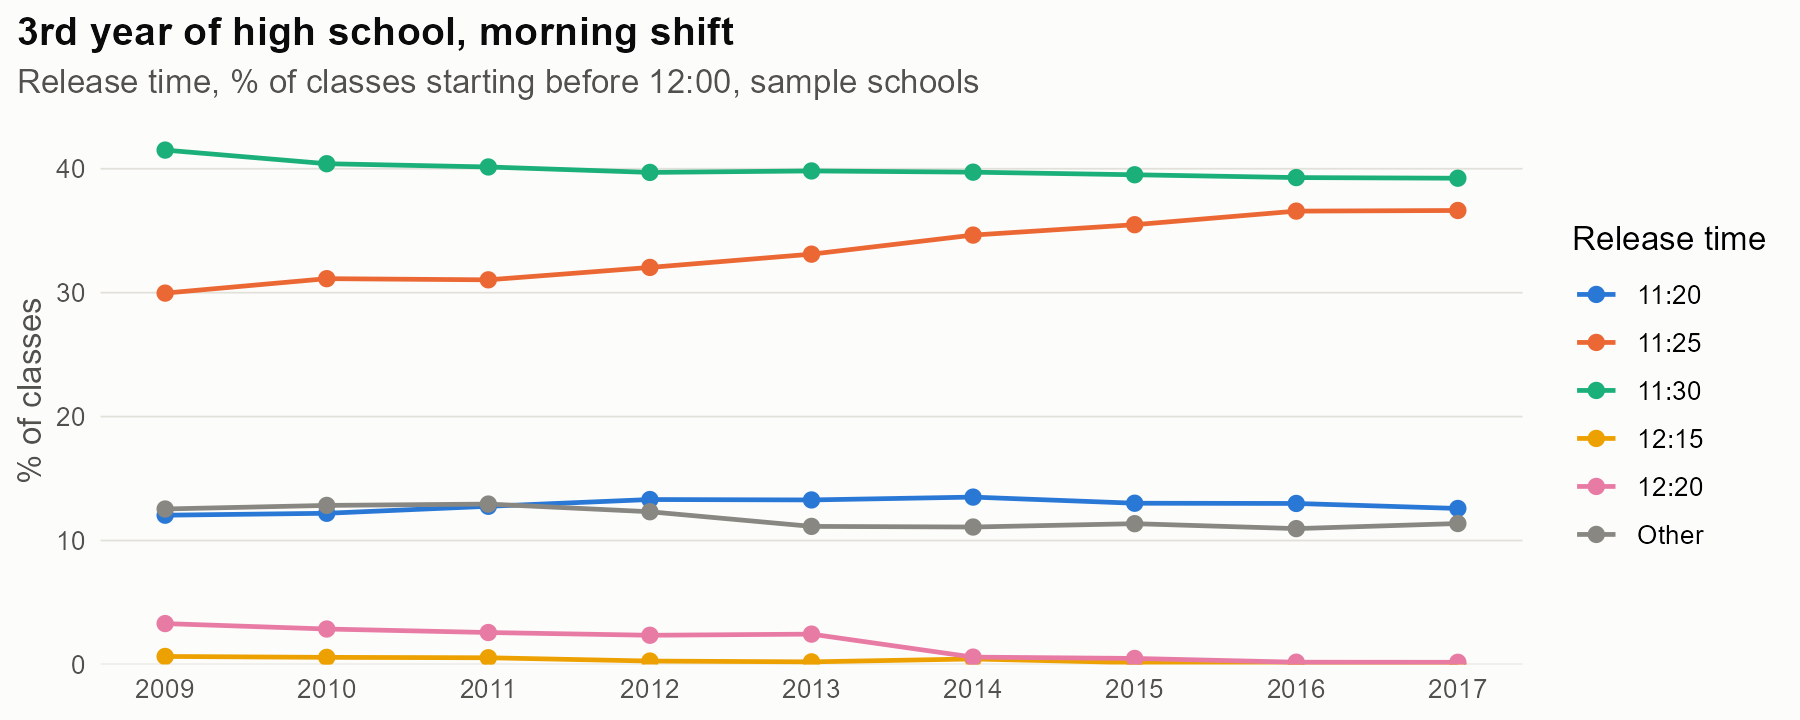
\includegraphics[width=0.85\textwidth]{horarios_em_series_manha_3ano.png}
\caption{Release time of EM classes in the morning shift (classes starting
before 12:00), by grade: 1st year (top), 2nd year (middle) and 3rd year
(bottom). Share of the grade's classes released at each time, by year. Sample
schools (Table~\ref{tab:escolas_2013}). The same release times, colors and
vertical axis are used in the three graphs; less frequent times are grouped as
Other.}
\label{fig:em_series_manha}
\end{figure}

\begin{figure}[htbp]
\centering
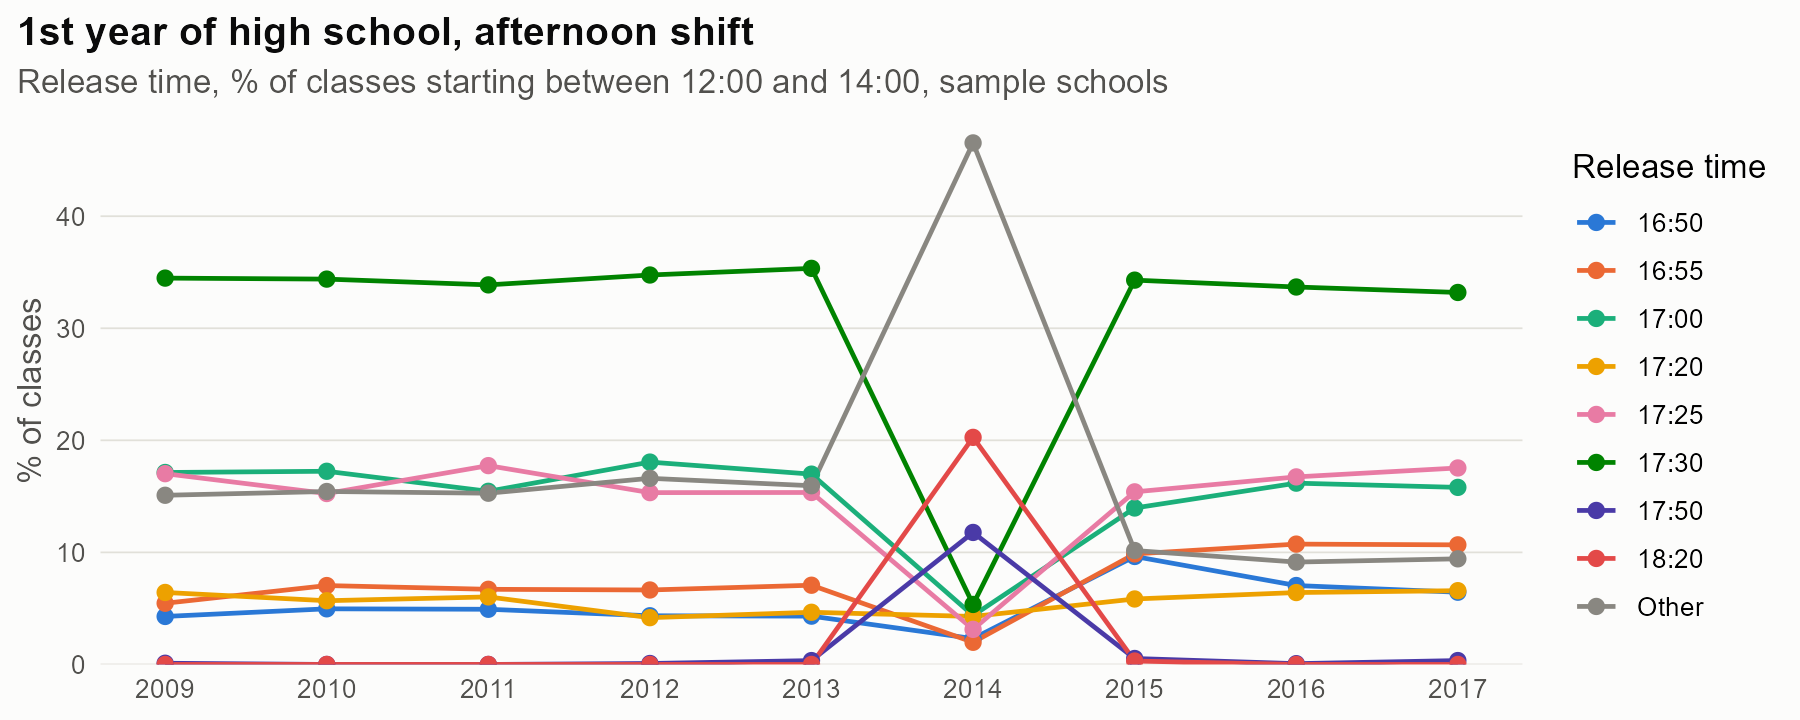
\includegraphics[width=0.85\textwidth]{horarios_em_series_tarde_1ano.png}\\[1ex]
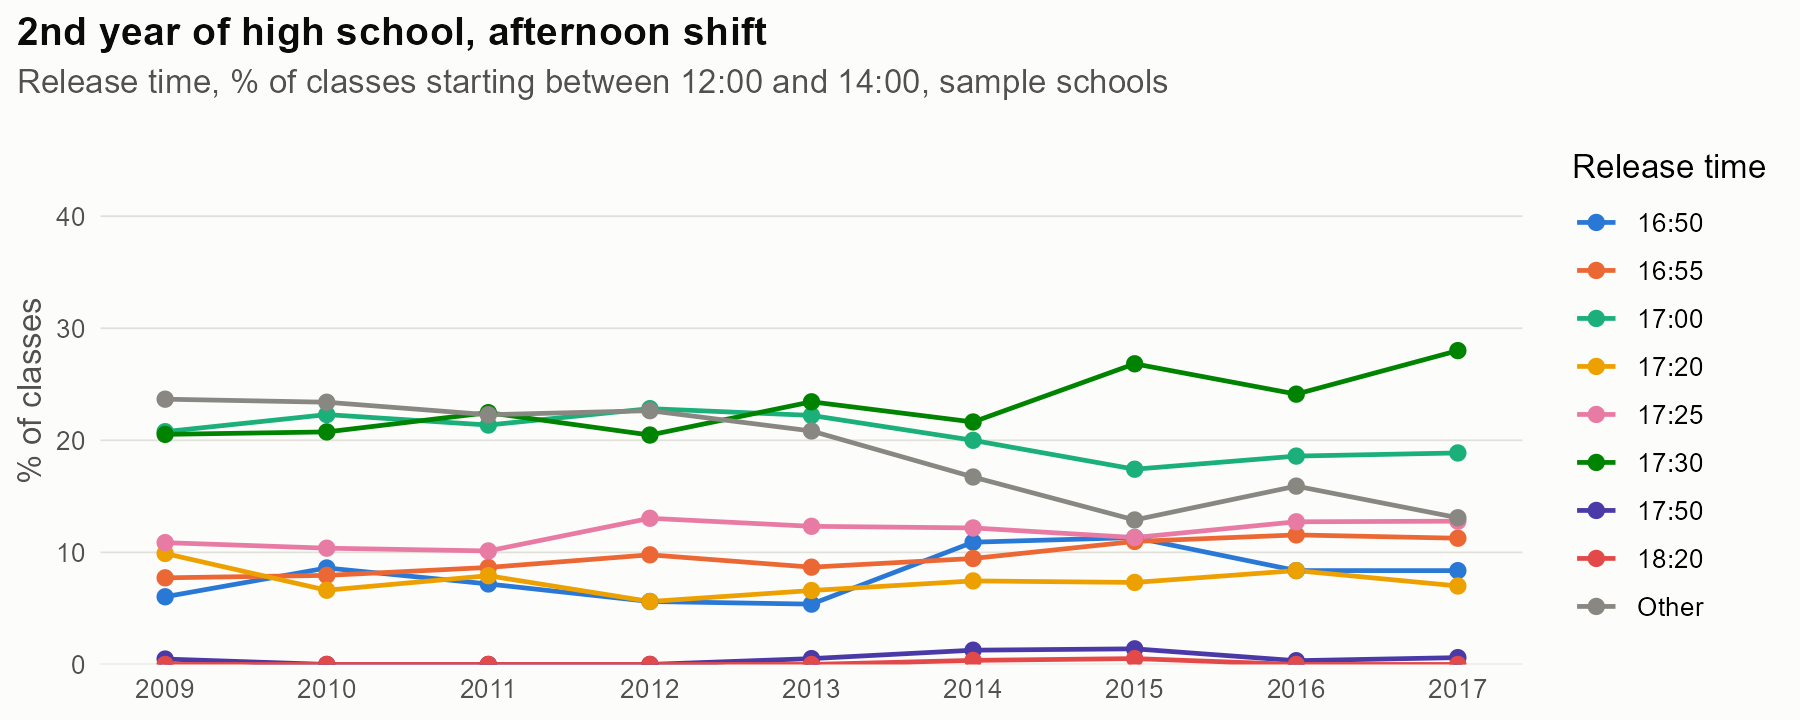
\includegraphics[width=0.85\textwidth]{horarios_em_series_tarde_2ano.png}\\[1ex]
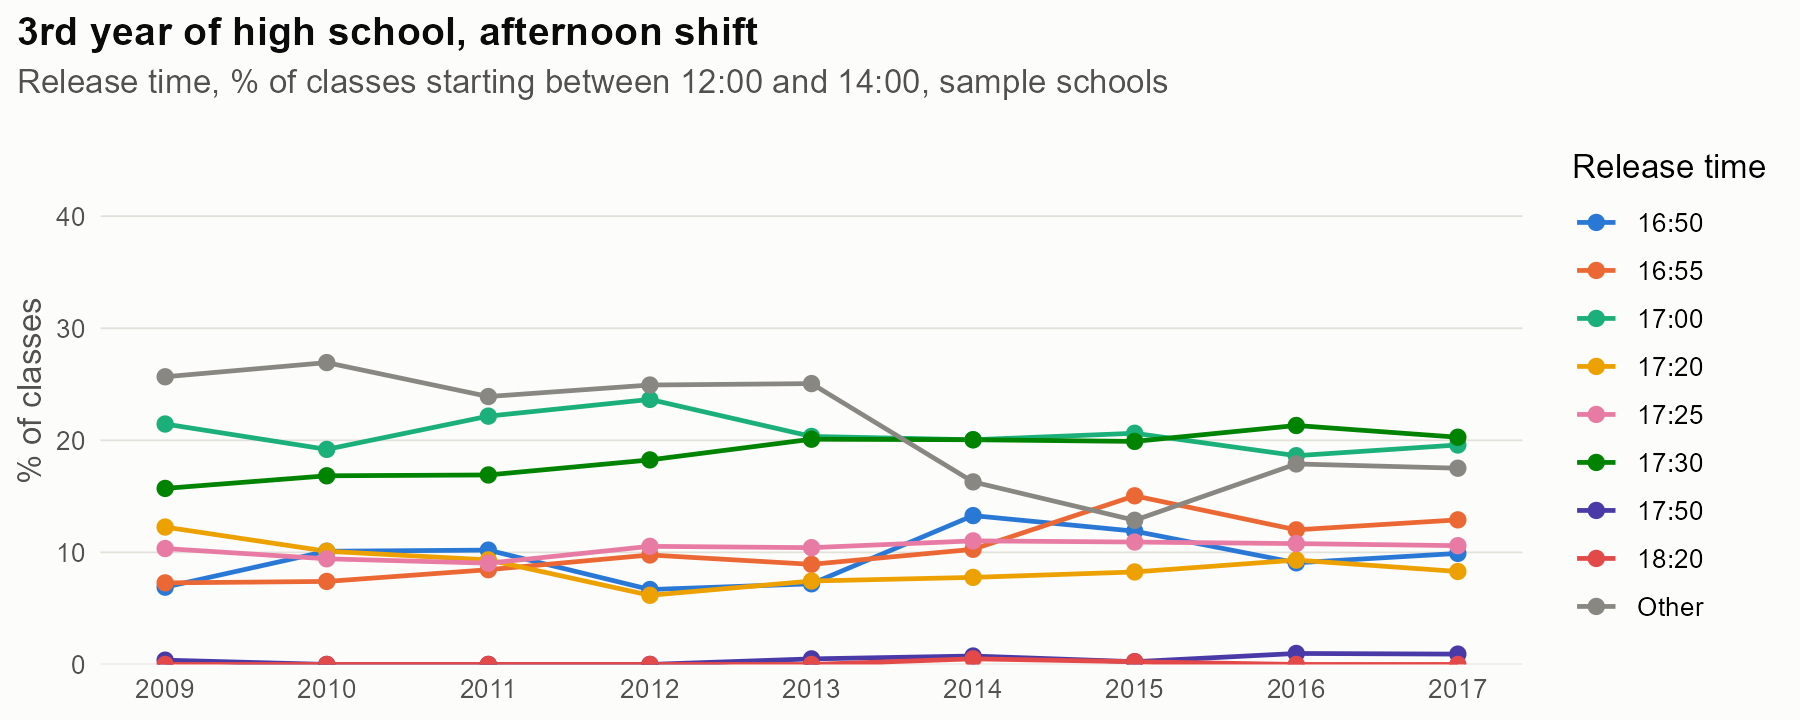
\includegraphics[width=0.85\textwidth]{horarios_em_series_tarde_3ano.png}
\caption{Release time of EM classes in the afternoon shift (classes starting
between 12:00 and 14:00), by grade: 1st year (top), 2nd year (middle) and 3rd
year (bottom). Share of the grade's classes released at each time, by year.
Sample schools (Table~\ref{tab:escolas_2013}). The same release times, colors
and vertical axis are used in the three graphs; less frequent times are grouped
as Other.}
\label{fig:em_series_tarde}
\end{figure}



\subsection{Backup sources of variation}

The main design rests on two assumptions: (i) without the 2014 change, crime
around the release of 2nd- and 3rd-year students would have evolved in parallel
in treated and control schools; (ii) the 2014 change reached these students only
through the number of students released with them. Its control group is also
small: in 2013, only 79 of the 1,766 comparable sample schools did not release
the 1st year within 5 minutes of the 2nd and 3rd years
(Table~\ref{tab:saida_junto}). Each design below relaxes part of this. In all of
them, $V_{jst}$ is crime by or against 2nd- and 3rd-year students of school $j$
after release in shift $s$ and year $t$.

\medskip
\noindent\textbf{(a) Schools that changed vs schools that did not change in 2014.}
\begin{itemize}
  \item \textbf{Comparison:} among schools that released the 1st year with the
        2nd and 3rd years in 2013, those whose 1st-year schedule changed in 2014
        (treated) vs those whose 1st-year schedule did not change (control:
        19.6\% of the sample have the same 1st-year class duration in 2013 and
        2014, Table~\ref{tab:escolas_2013}).
  \item \textbf{Unit and fixed effects:} school $\times$ shift $\times$ year;
        school $\times$ shift and year (regional office $\times$ year if the
        schools that did not change cluster in some regions).
  \item \textbf{Equation:} event study around 2014,
        \begin{equation}
          V_{jst} = \alpha_{js} + \lambda_t + \sum_{k \neq 2013} \beta_k\,
          \text{Change}_{js} \times \mathbf{1}[t=k] + \varepsilon_{jst}.
        \end{equation}
  \item \textbf{Identifying assumption:} without the 2014 change, schools that
        changed and schools that did not would have had parallel crime trends.
  \item \textbf{Violated if} the reason a school did not change its schedule
        (lack of rooms, a full-time program, a night shift, its regional office)
        also changes its crime trend. Check pre-trends in 2010--2013 and balance
        on size, location and region.
\end{itemize}

\medskip
\noindent\textbf{(b) Within school, across shifts.}
\begin{itemize}
  \item \textbf{Comparison:} in schools with EM in the morning and in the
        afternoon (19.5\% of the sample, Table~\ref{tab:escolas_2013}), the
        shift whose 1st year stopped leaving with the 2nd and 3rd years in 2014
        vs the shift where they kept leaving together.
  \item \textbf{Unit and fixed effects:} school $\times$ shift $\times$ year;
        school $\times$ year, school $\times$ shift and shift $\times$ year.
  \item \textbf{Equation:}
        \begin{equation}
          V_{jst} = \gamma_{jt} + \alpha_{js} + \delta_{st} + \beta\,
          \text{Lost}_{js} \times \mathbf{1}[t=2014] + \varepsilon_{jst},
        \end{equation}
        where $\text{Lost}_{js}=1$ if, in shift $s$ of school $j$, the 1st year
        stopped leaving with the 2nd and 3rd years in 2014.
  \item \textbf{Identifying assumption:} within a school, crime after release
        in the two shifts would have evolved in parallel.
  \item \textbf{What it adds:} school $\times$ year fixed effects absorb
        everything that changed at the school or in its neighborhood in 2014,
        including other parts of the program that reached all students.
  \item \textbf{Violated if} morning and afternoon trends differ for other
        reasons (who attends each shift, policing by time of day, World Cup
        match times), or students move between shifts because of the change.
        Spillover: in 2014 the morning 1st years leave at 12:15--12:20, close
        to when afternoon students arrive, so the afternoon shift may be
        affected by the morning change.
  \item \textbf{Feasibility:} count the schools in which the change differs
        between shifts.
\end{itemize}

\medskip
\noindent\textbf{(c) Intensity among schools that changed.}
\begin{itemize}
  \item \textbf{Comparison:} only schools that changed in 2014; those that lost
        a large 1st-year crowd vs those that lost a small one.
  \item \textbf{Treatment:} $N_{js}$, the number of 1st-year students who left
        within 5 minutes of the 2nd and 3rd years in shift $s$ of school $j$ in
        2013 (measured before the change).
  \item \textbf{Unit and fixed effects:} school $\times$ shift $\times$ year;
        school $\times$ shift and year.
  \item \textbf{Equation:}
        \begin{equation}
          V_{jst} = \alpha_{js} + \lambda_t + \beta\, N_{js} \times
          \mathbf{1}[t=2014] + \varepsilon_{jst}.
        \end{equation}
  \item \textbf{Identifying assumption:} among schools that changed, crime
        trends do not depend on the size of the 1st-year crowd they lost
        \citep[strong parallel trends;][]{callaway2024}.
  \item \textbf{What it adds:} the comparison does not use schools that did not
        change, and it gives a dose--response.
  \item \textbf{Violated if} the size of the 1st year tracks school size and
        density, whose areas have different crime trends; or if a large 1st
        year relative to the 3rd year signals repetition and dropout, that is,
        riskier students. Control for 2nd- and 3rd-year enrollment, or scale
        $N_{js}$ by it.
\end{itemize}

\medskip
\noindent\textbf{(d) The 2015 reversal, robust to linear trends.}
\begin{itemize}
  \item \textbf{Comparison:} each school's 2014 against the average of its 2013
        and 2015, treated vs control schools.
  \item \textbf{Unit and fixed effects:} school $\times$ shift $\times$ year;
        school $\times$ shift and year.
  \item \textbf{Estimator:}
        \begin{equation}
          \hat\beta = \Big[\overline{V}^{T}_{2014}
          - \tfrac{1}{2}\big(\overline{V}^{T}_{2013} + \overline{V}^{T}_{2015}\big)\Big]
          - \Big[\overline{V}^{C}_{2014}
          - \tfrac{1}{2}\big(\overline{V}^{C}_{2013} + \overline{V}^{C}_{2015}\big)\Big].
        \end{equation}
  \item \textbf{Identifying assumption:} in 2014, the deviation from a linear
        trend would be the same in treated and control schools. A linear trend
        that differs between the two groups cancels.
  \item \textbf{Violated if} the effect persists into 2015 (rivalries or
        partnerships formed in 2014), students anticipate the change in 2013,
        or a shock specific to 2014 hits the two groups differently.
\end{itemize}

\medskip
\noindent\textbf{(e) Time windows around the bell.} Needs geocoded crime
records with the time of the event.
\begin{itemize}
  \item \textbf{Comparison:} crime near the school in the window after the 2nd-
        and 3rd-year release vs other windows of the same day, on school days
        vs days without school (weekends, holidays, vacations), in 2014 vs 2013
        and 2015.
  \item \textbf{Unit and fixed effects:} school $\times$ 30-minute window
        $\times$ day; school $\times$ day, and school $\times$ window $\times$
        type of day (school day or not).
  \item \textbf{Identifying assumption:} a change in 2014 in crime that is
        specific to the release window \emph{and} to school days comes from the
        change in who is released.
  \item \textbf{What it adds:} school $\times$ day fixed effects absorb anything
        that hits the school's surroundings on that day; days without school
        absorb changes in policing or street activity at that hour.
  \item \textbf{Concentration test:} in 2014 the 1st year and the 2nd and 3rd
        years leave in two windows instead of one. If crime grows faster than
        the number of students released together, crime in the two windows in
        2014 adds up to less than crime in the single window of 2013 and 2015.
        If crime is proportional to the number of students, the sum does not
        change.
  \item \textbf{Violated if} police patrols follow the bell and changed in
        2014, or the school calendar changed (drop the World Cup weeks of
        June--July 2014). In the concentration test, the 1st years also leave
        later and after more hours in school, which changes their own crime.
\end{itemize}

\medskip
\noindent\textbf{(f) Student panel.} Needs a student identifier across years
and crime linked to students.
\begin{itemize}
  \item \textbf{Comparison:} the same students from the 2nd year (2013) to the
        3rd year (2014), in schools that changed vs schools that did not.
  \item \textbf{Unit and fixed effects:} student $\times$ year; student and
        year.
  \item \textbf{Identifying assumption:} moving from the 2nd to the 3rd year
        changes crime in the same way in both groups.
  \item \textbf{What it adds:} student fixed effects absorb the sorting of
        students into schools.
  \item \textbf{Violated if} dropout, repetition or changes of school depend on
        the treatment and are related to crime.
\end{itemize}

\medskip
\noindent\textbf{Estimators.} Treatment switches off in 2014 and back on in
2015, so two-way fixed effects can be biased when effects are heterogeneous; use
\citet{dechaisemartin2020}. If pre-trends fail, re-weight the control schools to
match the pre-2014 trends \citep[synthetic difference-in-differences;][]{arkhangelsky2021}
and report how large a violation of parallel trends would overturn the result
\citep{rambachan2023}. If only part of a school's 1st-year classes changed, use
the fuzzy version \citep{dechaisemartin2018}.

\medskip
\noindent\textbf{Which backup for which failure.}
\begin{itemize}
  \item Control schools trend differently: (a), (c), (d) and the estimators
        above.
  \item Something else changed at the school or in its neighborhood in 2014:
        (b) and (e).
  \item A statewide shock in 2014 (World Cup, elections) that hits treated and
        control schools differently: (e).
  \item Sorting of students into schools: (f).
\end{itemize}

\medskip
\noindent\textbf{Dropped from the 9th-grade version.} The within-school
comparison of classes released at different times (the earlier ``RCT'') has
little variation: only 6.2\% of the sample schools have different release times
within a grade and shift (Table~\ref{tab:escolas_2013}). Changes in shared
release in years other than 2014 appear to be rare (almost every school releases
all EM years together in 2013 and 2015, Figure~\ref{fig:hist_diff}), and they
are chosen by the school, which brings back reverse causality.








\bibliographystyle{aer}
\bibliography{references}
\end{document}
